\begin{filecontents*}[overwrite]{theme-showcase-bw.tex}
\documentclass[a4paper, 12pt, theme = bw]{../main/main}

\usepackage[utf8]{inputenc}
\usepackage[T1]{fontenc}

\usepackage[french]{babel, varioref}

\usepackage{enumitem}
\frenchsetup{StandardItemLabels=true}

\usepackage{tabularray}

\usepackage[lang = french]{tutodoc}


\usepackage{../admonitions/admonitions.cls}
\usepackage{../listing/listing.cls}
\usepackage{../version-n-change/version-n-change.cls}

\newcommand\thisstyle{bw}

\newcommand\myexarktext{
	\tdocdate{2024-10-23}
	Dans le cours du texte, il est utile d'indique des exemples et des remarques qui viennent compléter le contenu principal.
}

\newcommand\myadmotext{
	\tdocversion{1.6.0}[2024-10-23]
	Suivant le contexte d'utilisation, il est parfois utile de pouvoir mettre en vanat du contenu en indiquant au passage le degré d'importance qu'il faut apporter au contenu mis en exergue.
}

\newcommand\myhighlightedtext{
	Que dire
	\footnote{
		N'oublions les notes de bas de page...
	} ?
	Je ne sais pas, mais en tout cas, il semble utile de montrer ce que peut donner telle mise en forme, ou telle autre. Non ?
}

\begin{document}

{\Huge\bfseries Le thème \texttt{"\thisstyle"}}

\section{Mettre en avant, versionner et dater}

\ExplSyntaxOn

\seq_map_inline:Nn \__g_tutodoc_focus_std_seq {
	\subsection*{tdoc#1}

	\myexarktext

	\begin{tdoc#1}
		\myhighlightedtext
	\end{tdoc#1}
	
	\myexarktext
}

\ifcsundef{__g_tutodoc_focus_color_seq}{
	\prop_map_inline:Nn \__g_tutodoc_focus_color_prop {
    	\subsection*{tdoc#1}
    
    	\myadmotext
    	
    	\begin{tdoc#1}
    		\myhighlightedtext
    	\end{tdoc#1}
    	
    	\myadmotext
    }
} {
	\seq_map_inline:Nn \__g_tutodoc_focus_color_seq {
    	\subsection*{tdoc#1}
    
    	\myadmotext
    	
    	\begin{tdoc#1}
    		\myhighlightedtext
    	\end{tdoc#1}
    	
    	\myadmotext
    }
}

\ExplSyntaxOff

\section{Des codes \LaTeX}

Il est aussi utile de pouvoir montrer des cas d'utilisation en \LaTeX.

\begin{tdoclatex}
Voir du code \LaTeX\ mis en forme, c'est sympa : $E = m c^2$ ou $\pi \neq \frac{3}{14}$.
\end{tdoclatex}


On peut utiliser un monde côte-à-côte. Sympa ! Non ? 

\begin{tdoclatex}[sbs]
Voir du code \LaTeX\ mis en forme, 
c'est sympa : $E = m c^2$ ou 
$\pi \neq \frac{3}{14}$.
\end{tdoclatex}

\end{document}

\end{filecontents*}

\begin{filecontents*}[overwrite]{theme-showcase-color.tex}
\documentclass[a4paper, 12pt, theme = color]{../main/main}

\usepackage[utf8]{inputenc}
\usepackage[T1]{fontenc}

\usepackage[french]{babel, varioref}

\usepackage{enumitem}
\frenchsetup{StandardItemLabels=true}

\usepackage{tabularray}

\usepackage[lang = french]{tutodoc}


\usepackage{../admonitions/admonitions.cls}
\usepackage{../listing/listing.cls}
\usepackage{../version-n-change/version-n-change.cls}

\newcommand\thisstyle{color}

\newcommand\myexarktext{
	\tdocdate{2024-10-23}
	Dans le cours du texte, il est utile d'indique des exemples et des remarques qui viennent compléter le contenu principal.
}

\newcommand\myadmotext{
	\tdocversion{1.6.0}[2024-10-23]
	Suivant le contexte d'utilisation, il est parfois utile de pouvoir mettre en vanat du contenu en indiquant au passage le degré d'importance qu'il faut apporter au contenu mis en exergue.
}

\newcommand\myhighlightedtext{
	Que dire
	\footnote{
		N'oublions les notes de bas de page...
	} ?
	Je ne sais pas, mais en tout cas, il semble utile de montrer ce que peut donner telle mise en forme, ou telle autre. Non ?
}

\begin{document}

{\Huge\bfseries Le thème \texttt{"\thisstyle"}}

\section{Mettre en avant, versionner et dater}

\ExplSyntaxOn

\seq_map_inline:Nn \__g_tutodoc_focus_std_seq {
	\subsection*{tdoc#1}

	\myexarktext

	\begin{tdoc#1}
		\myhighlightedtext
	\end{tdoc#1}
	
	\myexarktext
}

\ifcsundef{__g_tutodoc_focus_color_seq}{
	\prop_map_inline:Nn \__g_tutodoc_focus_color_prop {
    	\subsection*{tdoc#1}
    
    	\myadmotext
    	
    	\begin{tdoc#1}
    		\myhighlightedtext
    	\end{tdoc#1}
    	
    	\myadmotext
    }
} {
	\seq_map_inline:Nn \__g_tutodoc_focus_color_seq {
    	\subsection*{tdoc#1}
    
    	\myadmotext
    	
    	\begin{tdoc#1}
    		\myhighlightedtext
    	\end{tdoc#1}
    	
    	\myadmotext
    }
}

\ExplSyntaxOff

\section{Des codes \LaTeX}

Il est aussi utile de pouvoir montrer des cas d'utilisation en \LaTeX.

\begin{tdoclatex}
Voir du code \LaTeX\ mis en forme, c'est sympa : $E = m c^2$ ou $\pi \neq \frac{3}{14}$.
\end{tdoclatex}


On peut utiliser un monde côte-à-côte. Sympa ! Non ? 

\begin{tdoclatex}[sbs]
Voir du code \LaTeX\ mis en forme, 
c'est sympa : $E = m c^2$ ou 
$\pi \neq \frac{3}{14}$.
\end{tdoclatex}

\end{document}

\end{filecontents*}

\begin{filecontents*}[overwrite]{theme-showcase-dark.tex}
\documentclass[a4paper, 12pt, theme = dark]{../main/main}

\usepackage[utf8]{inputenc}
\usepackage[T1]{fontenc}

\usepackage[french]{babel, varioref}

\usepackage{enumitem}
\frenchsetup{StandardItemLabels=true}

\usepackage{tabularray}

\usepackage[lang = french]{tutodoc}


\usepackage{../admonitions/admonitions.cls}
\usepackage{../listing/listing.cls}
\usepackage{../version-n-change/version-n-change.cls}

\newcommand\thisstyle{dark}

\newcommand\myexarktext{
	\tdocdate{2024-10-23}
	Dans le cours du texte, il est utile d'indique des exemples et des remarques qui viennent compléter le contenu principal.
}

\newcommand\myadmotext{
	\tdocversion{1.6.0}[2024-10-23]
	Suivant le contexte d'utilisation, il est parfois utile de pouvoir mettre en vanat du contenu en indiquant au passage le degré d'importance qu'il faut apporter au contenu mis en exergue.
}

\newcommand\myhighlightedtext{
	Que dire
	\footnote{
		N'oublions les notes de bas de page...
	} ?
	Je ne sais pas, mais en tout cas, il semble utile de montrer ce que peut donner telle mise en forme, ou telle autre. Non ?
}

\begin{document}

{\Huge\bfseries Le thème \texttt{"\thisstyle"}}

\section{Mettre en avant, versionner et dater}

\ExplSyntaxOn

\seq_map_inline:Nn \__g_tutodoc_focus_std_seq {
	\subsection*{tdoc#1}

	\myexarktext

	\begin{tdoc#1}
		\myhighlightedtext
	\end{tdoc#1}
	
	\myexarktext
}

\ifcsundef{__g_tutodoc_focus_color_seq}{
	\prop_map_inline:Nn \__g_tutodoc_focus_color_prop {
    	\subsection*{tdoc#1}
    
    	\myadmotext
    	
    	\begin{tdoc#1}
    		\myhighlightedtext
    	\end{tdoc#1}
    	
    	\myadmotext
    }
} {
	\seq_map_inline:Nn \__g_tutodoc_focus_color_seq {
    	\subsection*{tdoc#1}
    
    	\myadmotext
    	
    	\begin{tdoc#1}
    		\myhighlightedtext
    	\end{tdoc#1}
    	
    	\myadmotext
    }
}

\ExplSyntaxOff

\section{Des codes \LaTeX}

Il est aussi utile de pouvoir montrer des cas d'utilisation en \LaTeX.

\begin{tdoclatex}
Voir du code \LaTeX\ mis en forme, c'est sympa : $E = m c^2$ ou $\pi \neq \frac{3}{14}$.
\end{tdoclatex}


On peut utiliser un monde côte-à-côte. Sympa ! Non ? 

\begin{tdoclatex}[sbs]
Voir du code \LaTeX\ mis en forme, 
c'est sympa : $E = m c^2$ ou 
$\pi \neq \frac{3}{14}$.
\end{tdoclatex}

\end{document}

\end{filecontents*}

\begin{filecontents*}[overwrite]{theme-showcase-draft.tex}
\documentclass[a4paper, 12pt, theme = draft]{../main/main}

\usepackage[utf8]{inputenc}
\usepackage[T1]{fontenc}

\usepackage[french]{babel, varioref}

\usepackage{enumitem}
\frenchsetup{StandardItemLabels=true}

\usepackage{tabularray}

\usepackage[lang = french]{tutodoc}


\usepackage{../admonitions/admonitions.cls}
\usepackage{../listing/listing.cls}
\usepackage{../version-n-change/version-n-change.cls}

\newcommand\thisstyle{draft}

\newcommand\myexarktext{
	\tdocdate{2024-10-23}
	Dans le cours du texte, il est utile d'indique des exemples et des remarques qui viennent compléter le contenu principal.
}

\newcommand\myadmotext{
	\tdocversion{1.6.0}[2024-10-23]
	Suivant le contexte d'utilisation, il est parfois utile de pouvoir mettre en vanat du contenu en indiquant au passage le degré d'importance qu'il faut apporter au contenu mis en exergue.
}

\newcommand\myhighlightedtext{
	Que dire
	\footnote{
		N'oublions les notes de bas de page...
	} ?
	Je ne sais pas, mais en tout cas, il semble utile de montrer ce que peut donner telle mise en forme, ou telle autre. Non ?
}

\begin{document}

{\Huge\bfseries Le thème \texttt{"\thisstyle"}}

\section{Mettre en avant, versionner et dater}

\ExplSyntaxOn

\seq_map_inline:Nn \__g_tutodoc_focus_std_seq {
	\subsection*{tdoc#1}

	\myexarktext

	\begin{tdoc#1}
		\myhighlightedtext
	\end{tdoc#1}
	
	\myexarktext
}

\ifcsundef{__g_tutodoc_focus_color_seq}{
	\prop_map_inline:Nn \__g_tutodoc_focus_color_prop {
    	\subsection*{tdoc#1}
    
    	\myadmotext
    	
    	\begin{tdoc#1}
    		\myhighlightedtext
    	\end{tdoc#1}
    	
    	\myadmotext
    }
} {
	\seq_map_inline:Nn \__g_tutodoc_focus_color_seq {
    	\subsection*{tdoc#1}
    
    	\myadmotext
    	
    	\begin{tdoc#1}
    		\myhighlightedtext
    	\end{tdoc#1}
    	
    	\myadmotext
    }
}

\ExplSyntaxOff

\section{Des codes \LaTeX}

Il est aussi utile de pouvoir montrer des cas d'utilisation en \LaTeX.

\begin{tdoclatex}
Voir du code \LaTeX\ mis en forme, c'est sympa : $E = m c^2$ ou $\pi \neq \frac{3}{14}$.
\end{tdoclatex}


On peut utiliser un monde côte-à-côte. Sympa ! Non ? 

\begin{tdoclatex}[sbs]
Voir du code \LaTeX\ mis en forme, 
c'est sympa : $E = m c^2$ ou 
$\pi \neq \frac{3}{14}$.
\end{tdoclatex}

\end{document}

\end{filecontents*}

\documentclass[10pt, a4paper]{../main/main}

\usepackage[utf8]{inputenc}
\usepackage[T1]{fontenc}

\usepackage[french]{babel, varioref}

\usepackage{enumitem}
\frenchsetup{StandardItemLabels=true}

\usepackage{tabularray}

\usepackage[lang = french]{tutodoc}


\begin{document}

\immediate\write18{pdflatex -shell-escape theme-showcase-bw}

\immediate\write18{pdflatex -shell-escape theme-showcase-color}

\immediate\write18{pdflatex -shell-escape theme-showcase-dark}

\immediate\write18{pdflatex -shell-escape theme-showcase-draft}

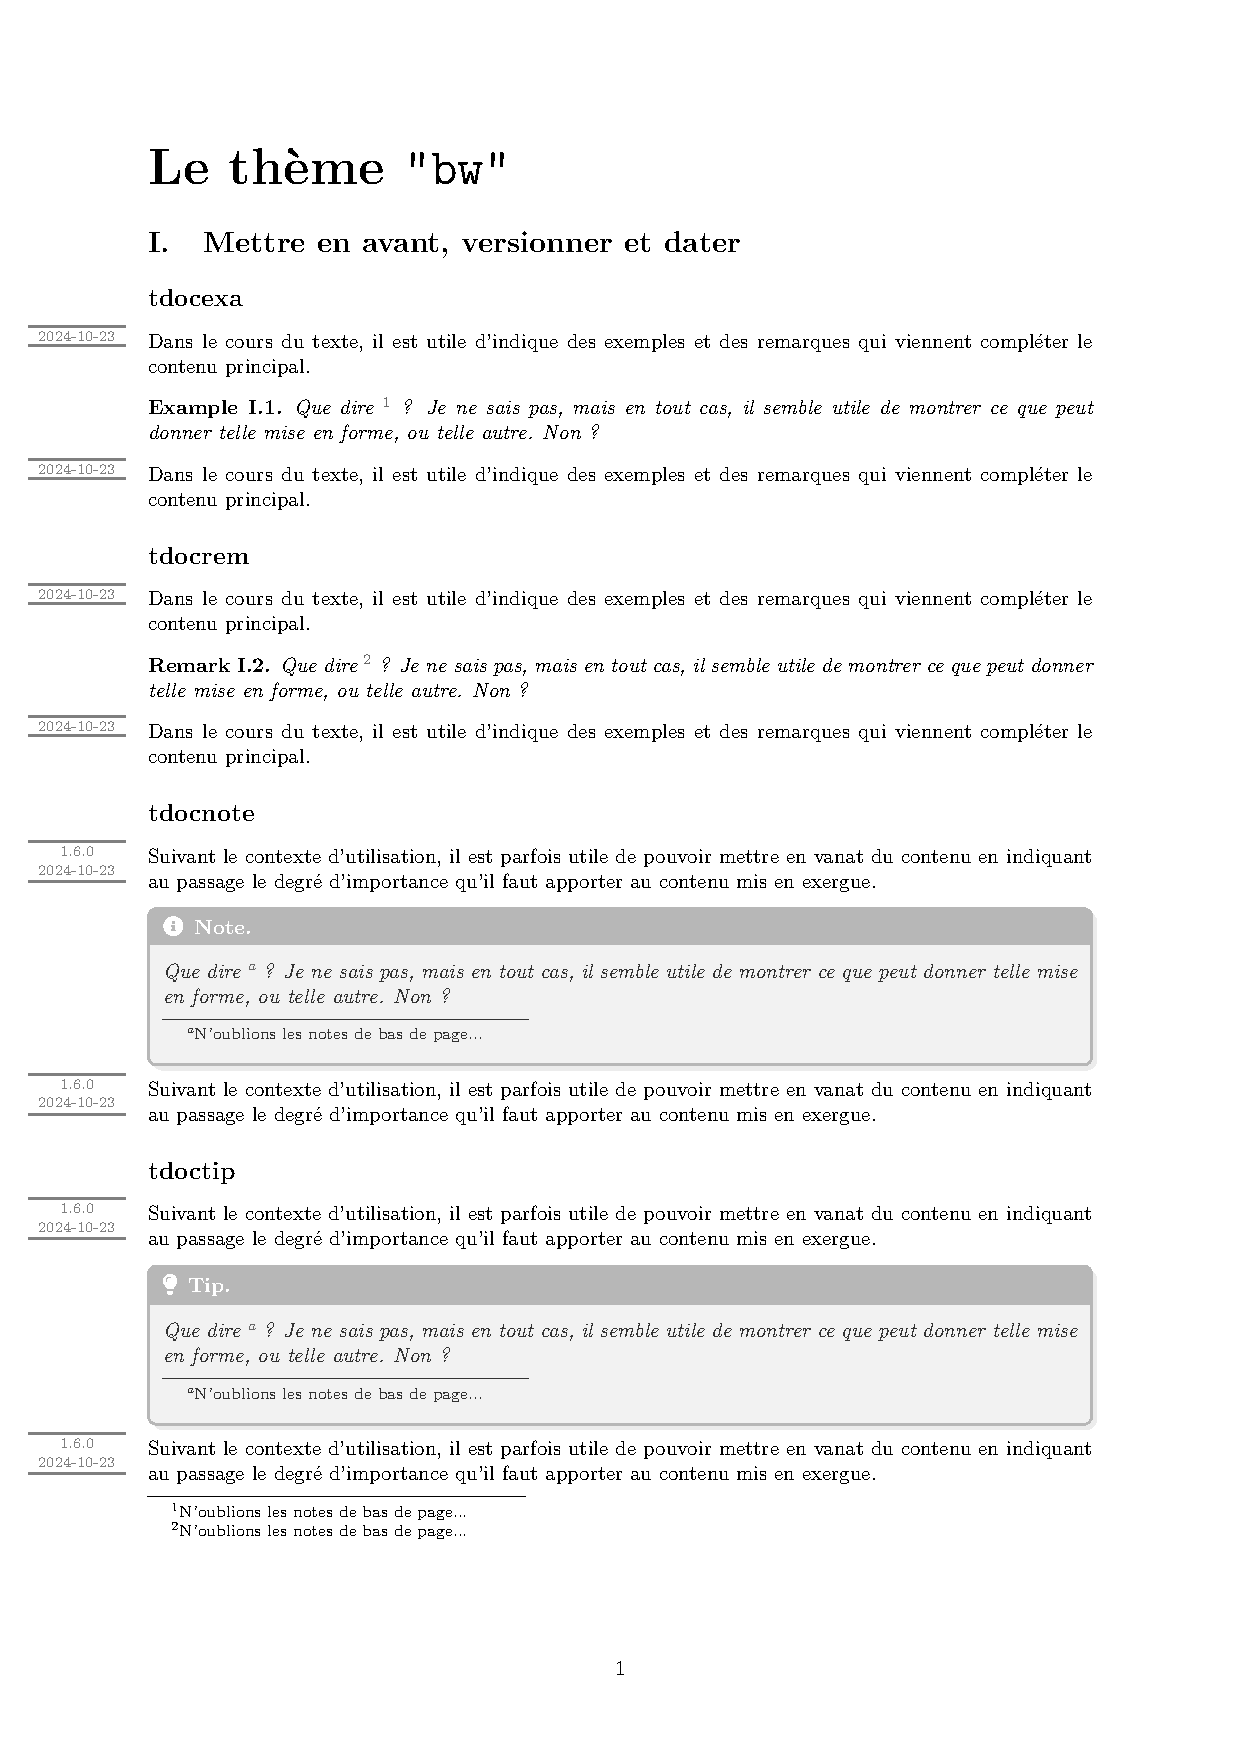
\includepdf[
	pages=1-2,
	fitpaper=true
]{theme-showcase-bw}

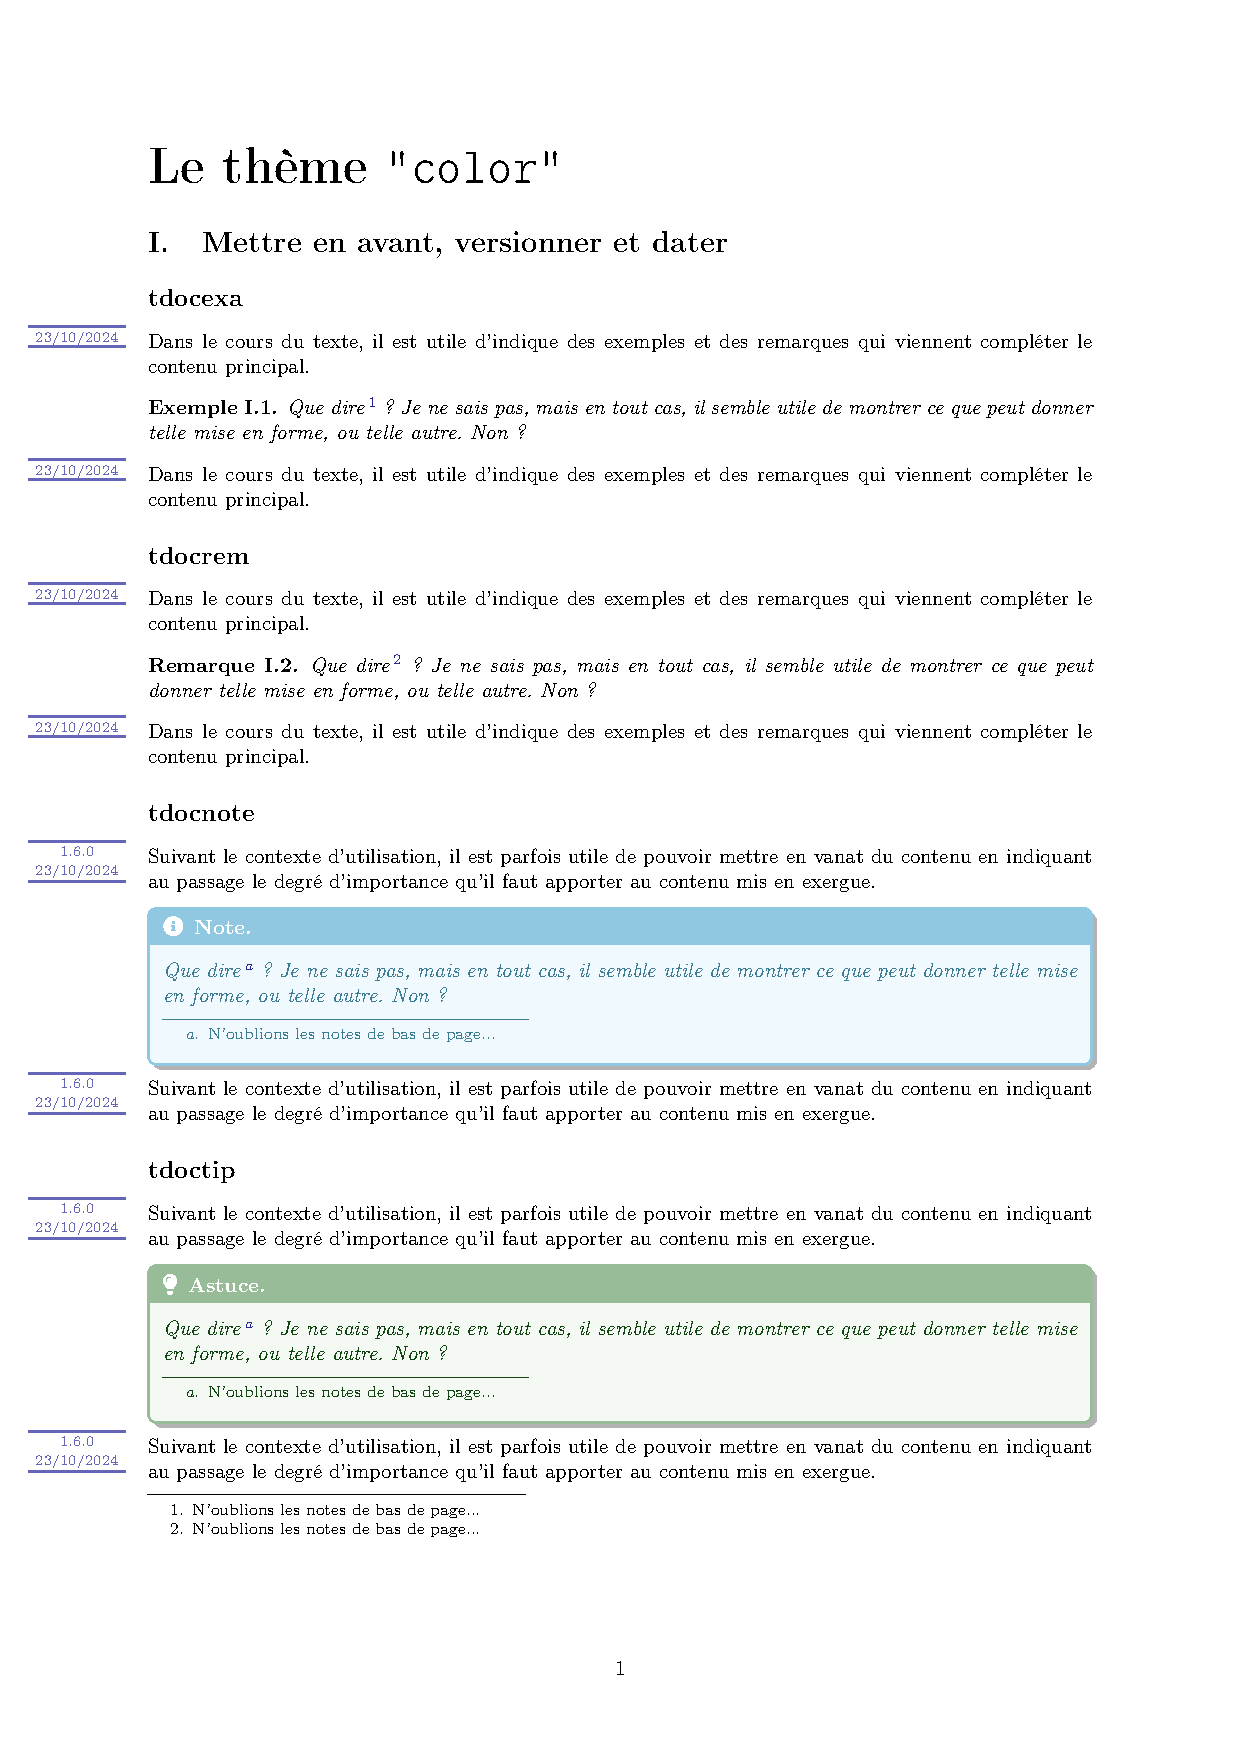
\includepdf[
	pages=1-2,
	fitpaper=true
]{theme-showcase-color}

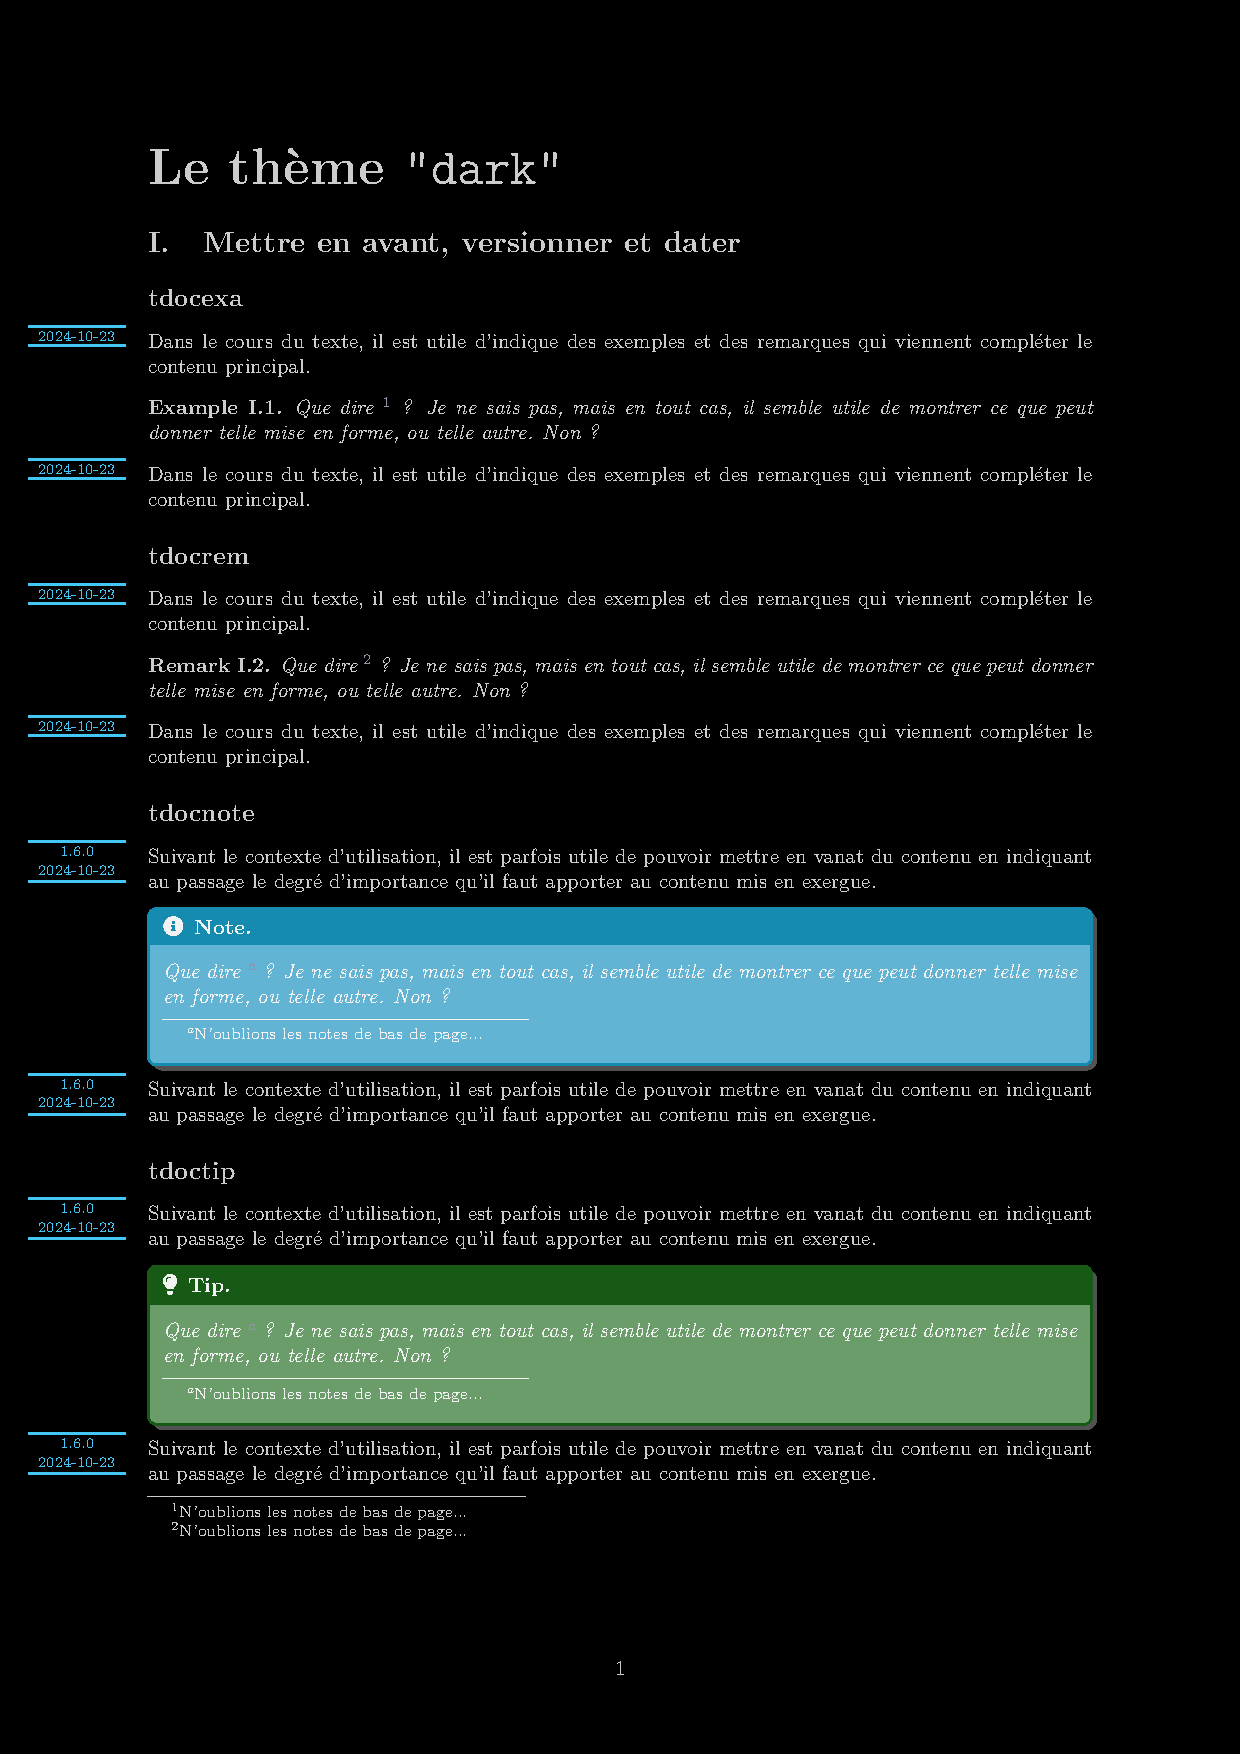
\includepdf[
	pages=1-2,
	fitpaper=true
]{theme-showcase-dark}

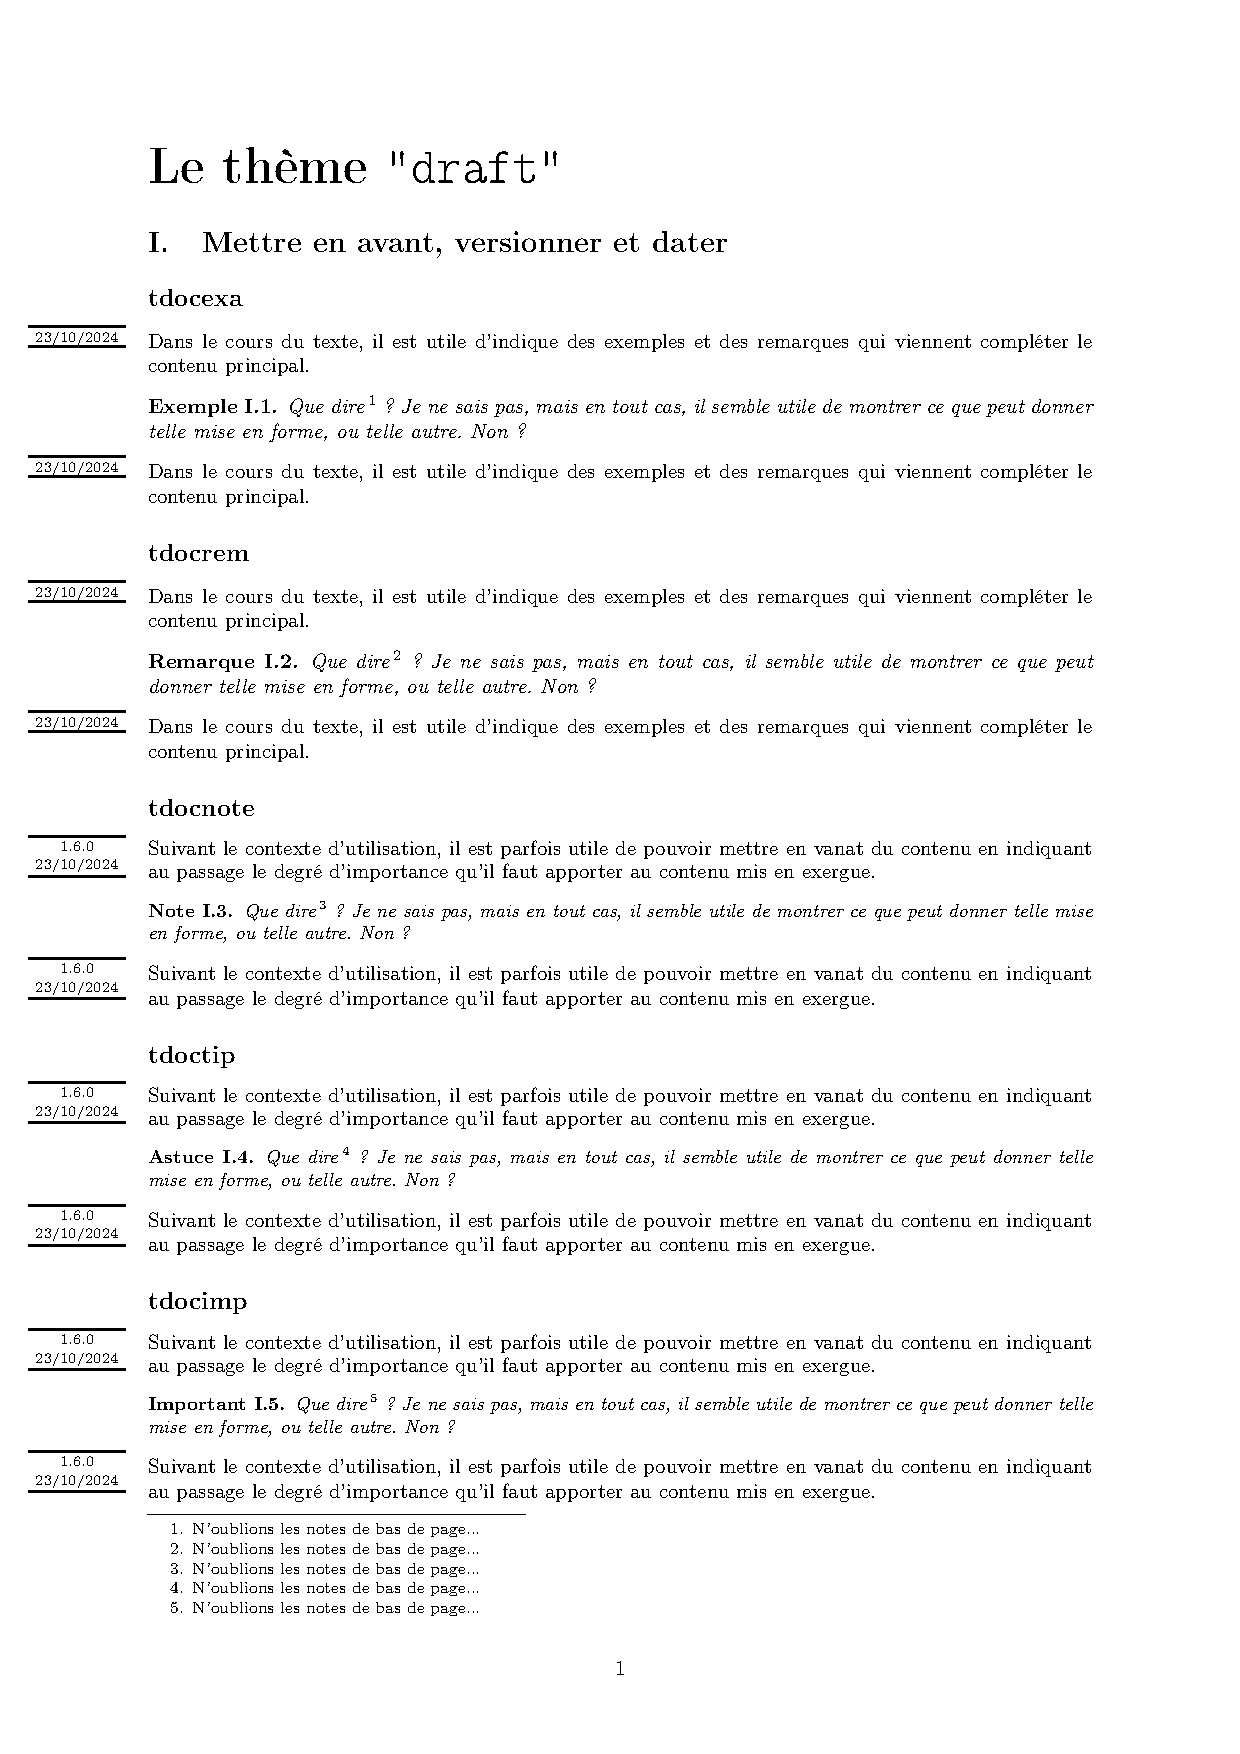
\includepdf[
	pages=1-2,
	fitpaper=true
]{theme-showcase-draft}

\end{document}
